\section{Electron neutrino scattering cross section.}

\begin{enumerate}[label=\textbf{\alph*}.]
  \item Assuming that the process $\nu_e e^- \to e^- \nu_e$ only occurs by the weak charged-current interaction (ignore $Z$), show that $\sigma_{CC}^{\nu_e e^-} \approx \frac{2m_e E_\nu G_F^2}{\pi}$, where $E_\nu$ is in the lab frame where the struck $e^-$ is at rest.

  Remember in chapter 12.2 when we derived the charged-current cross section of neutrino scattering off a nucleus? Let's try to do something similar here.

  We have a feynman diagram like the middle bit of Thomson figure 12.4, just with $d=\mu^-, u=\nu_\mu$ and $\mu=e$.

  \begin{center}
    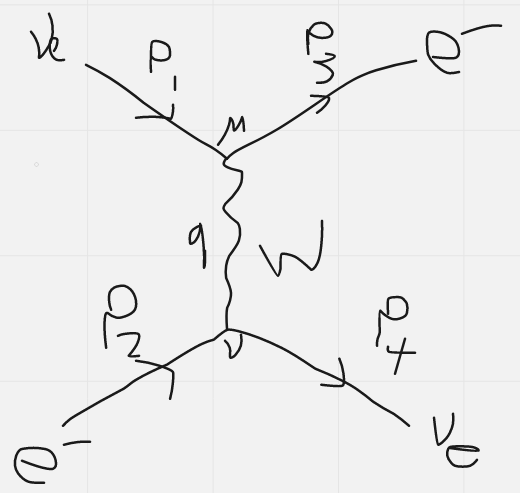
\includegraphics[width=0.5\textwidth]{q4_feynman.png}
  \end{center}

  For a neutrino interacting with an electron at rest, the CoM energy squared is $s = (p_1 + p_2)^2 = (E_\nu + m_e)^2 - E_\nu^2 = 2m_e E_\nu + m_e^2$. For high-energy neutrinos we can ignore the $m_e^2$ term and just say $s = 2m_e E_\nu$.

  Calculate the matrix element here, ignoring $q^2$ dependence as in 12.2.1:

  \begin{itemize}
    \item Incoming $\nu_e$: $u(p_1)$
    \item Outgoing $e^-$: $\bar{u}(p_3)$
    \item $W^-$ propagator: appx $\frac{-ig_{\mu\nu}}{m_W^2}$
    \item $e^- \to W^- \nu_e$ vertex 1: $\frac{-ig_w}{\sqrt{2}}\frac{1}{2}\gamma^\mu(1-\gamma^5)$
    \item $e^- \to W^- \nu_e$ vertex 2: $\frac{-ig_w}{\sqrt{2}}\frac{1}{2}\gamma^\nu(1-\gamma^5)$
    \item Incoming $e^-$: $u(p_2)$
    \item Outgoing $\nu_e$: $\bar{u}(p_4)$
  \end{itemize}

  \begin{align*}
    -iM_{fi} &= \left[\bar{u}(p_3)\frac{-ig_w}{\sqrt{2}}\frac{1}{2}\gamma^\mu(1-\gamma^5)u(p_1)\right]\frac{-ig_{\mu\nu}}{m_W^2}\left[\bar{u}(p_4)\frac{-ig_w}{\sqrt{2}}\frac{1}{2}\gamma^\nu(1-\gamma^5)u(p_2)\right] \\
    M_{fi} &= \frac{g_w^2}{2m_W^2}g_{\mu\nu}\left[\bar{u}(p_3)\gamma^\mu\frac{1}{2}(1-\gamma^5)u(p_1)\right]\left[\bar{u}(p_4)\gamma^\nu\frac{1}{2}(1-\gamma^5)u(p_2)\right] \\
  \end{align*}

  For high-energy neutrino scattering, let's approximate chiral states = helicity states, and from here the calculation of $\sigma$ is exactly the same as in 12.2.1, yielding

  $$\sigma_{CC}(\nu_e e^- \to \nu_e e^-) = \frac{G_F^2s}{\pi}.$$

  Using our $s = 2m_e E_\nu$, we find what the question wanted us to show:

  $$\sigma_{CC}^{\nu_e e^-} \approx \frac{2m_e E_\nu G_F^2}{\pi}$$

  \item Using the above result, estimate the probability that a $\SI{10}{MeV}$ solar electron neutrino will undergo a charged-current weak interaction with an electron in the earth if it travels along a trajectory passing through the centre of the earth. Take the earth to be a sphere of radius $R=\SI{6400}{km}$ and uniform density $\rho = \SI{5520}{kgm^{-3}}$.

  To get the probability of an interaction (which we know will be relatively small), we can use $\sigma = \frac{P}{n_e}$, where $n_e$ is the surface area number density of electrons in our path, i.e. $n_e = N_e/A$.

  Consider the cross section first:
  \begin{align*}
    \sigma_{CC}^{\nu_e e^-} &= \frac{2m_e E_\nu G_F^2}{\pi} \\
  \end{align*}
  
  \begin{align*}
    G_F &= \SI{1.16638e-5}{GeV^{-2}}
  \end{align*}

  Mass volume density is $\rho$, get mass are density:
  \begin{align*}
    M/A &= \rho d\\
    &= \rho 2R\\
  \end{align*}

  Some fraction of the mass of the earth is due to electrons, say $\frac{1}{2000}$ since the earth is mostly compoased of atoms with equal amounts of neutrons and protons, and $m_e \approx \frac{1}{1000} m_p$.

  \begin{align*}
    M_e/A &= \frac{1}{1000}\rho R\\
  \end{align*}

  The electron mass here can be written as $M_e = N_e m_e$,

  \begin{align*}
    N_e m_e/A &= \frac{1}{1000}\rho R\\
    n_e m_e &= \frac{1}{1000}\rho R\\
    n_e &= \frac{1}{m_e}\frac{1}{1000}\rho R\\
    &= \SI{3.8781987e37}{m^{-2}}
  \end{align*}

  Use this to get the probability we're after:
  \begin{align*}
    P &= \sigma n_e \\
    &= \frac{2m_e E_\nu G_F^2}{\pi} n_e \\
    &= \frac{2E_\nu G_F^2}{\pi} \frac{1}{1000}\rho R\\
    &= \frac{2(\SI{10}{MeV}) (\SI{1.16638e-5}{GeV^{-2}})^2}{\pi} \frac{1}{1000}\SI{5520}{kgm^{-3}}\SI{6400}{km} \\
    &= \SI{6.68e-10}{}
  \end{align*}
  (There were some extra factors in there from implicit $\hbar$s and $c$s. In the spirit of natural units, I've left those out.)

\end{enumerate}

